%\section*{\begin{center}{\Huge Appendix}\end{center}}
\addcontentsline{toc}{chapter}{Appendix}
\chapter{Plots}\label{Appendix}

\section{Per seed plots of experiments}

\subsection{Corridor}

\begin{figure}[H]
    \centering
    \subfloat[DQN]{
        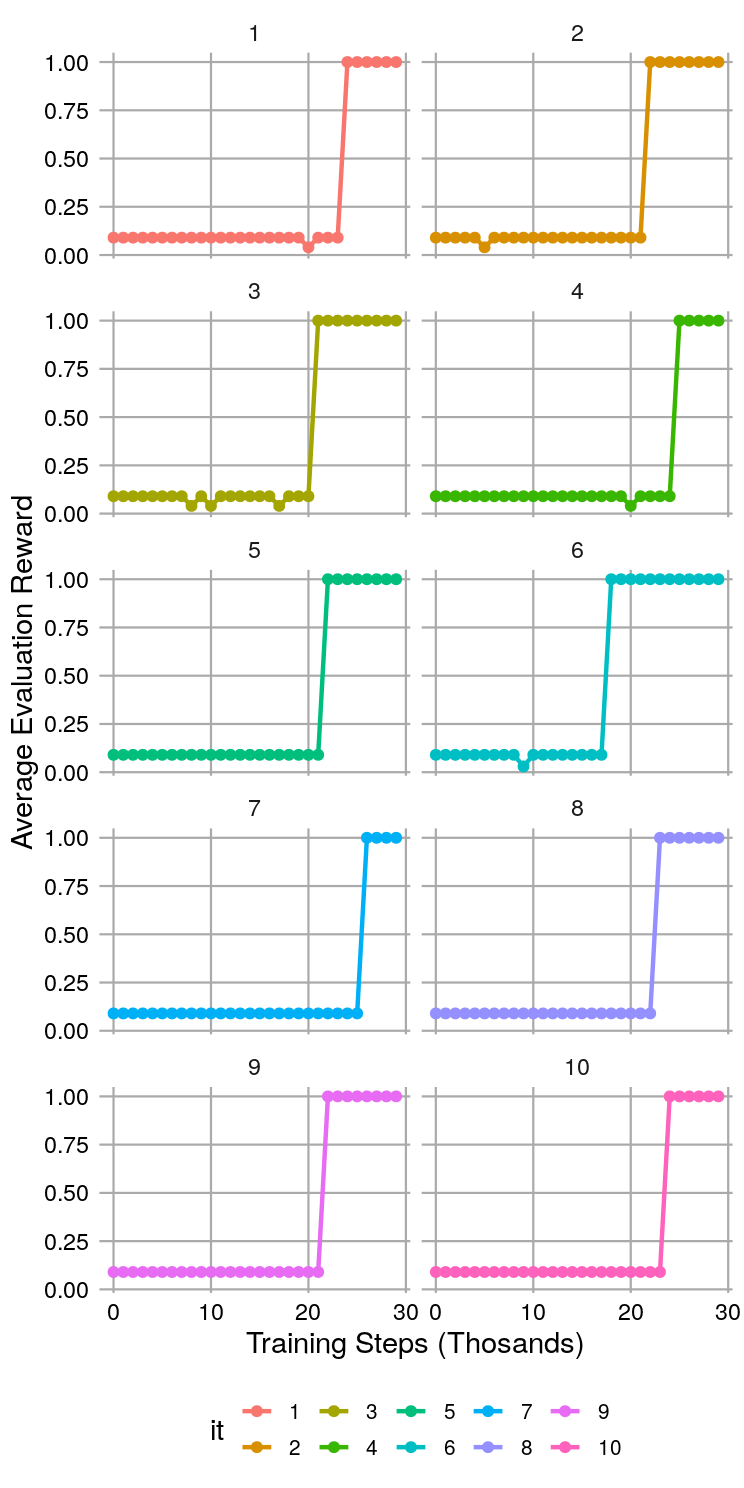
\includegraphics[scale=0.5]{PerDQNCorridor.png}
    }
    \subfloat[BNIG DQN]{
        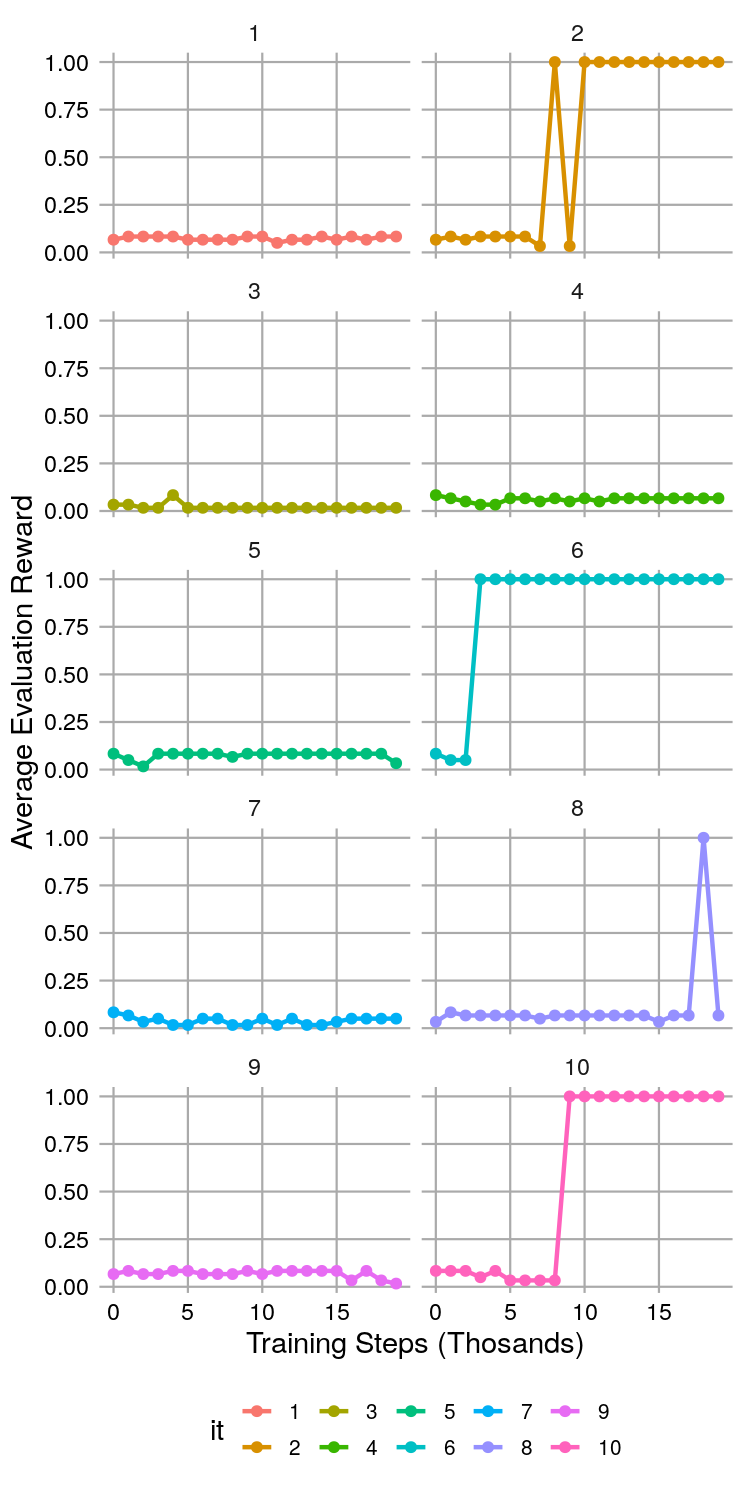
\includegraphics[scale=0.5]{PerBDQNCorridor.png}
    }
    \caption{\textbf{Per Seed DQN and BNIG DQN Performance on Corridor}}
    \label{fig:nn_per_cartpole}
\end{figure}

\subsection{Cartpole}

\begin{figure}[H]
    \centering
    \subfloat[DQN]{
        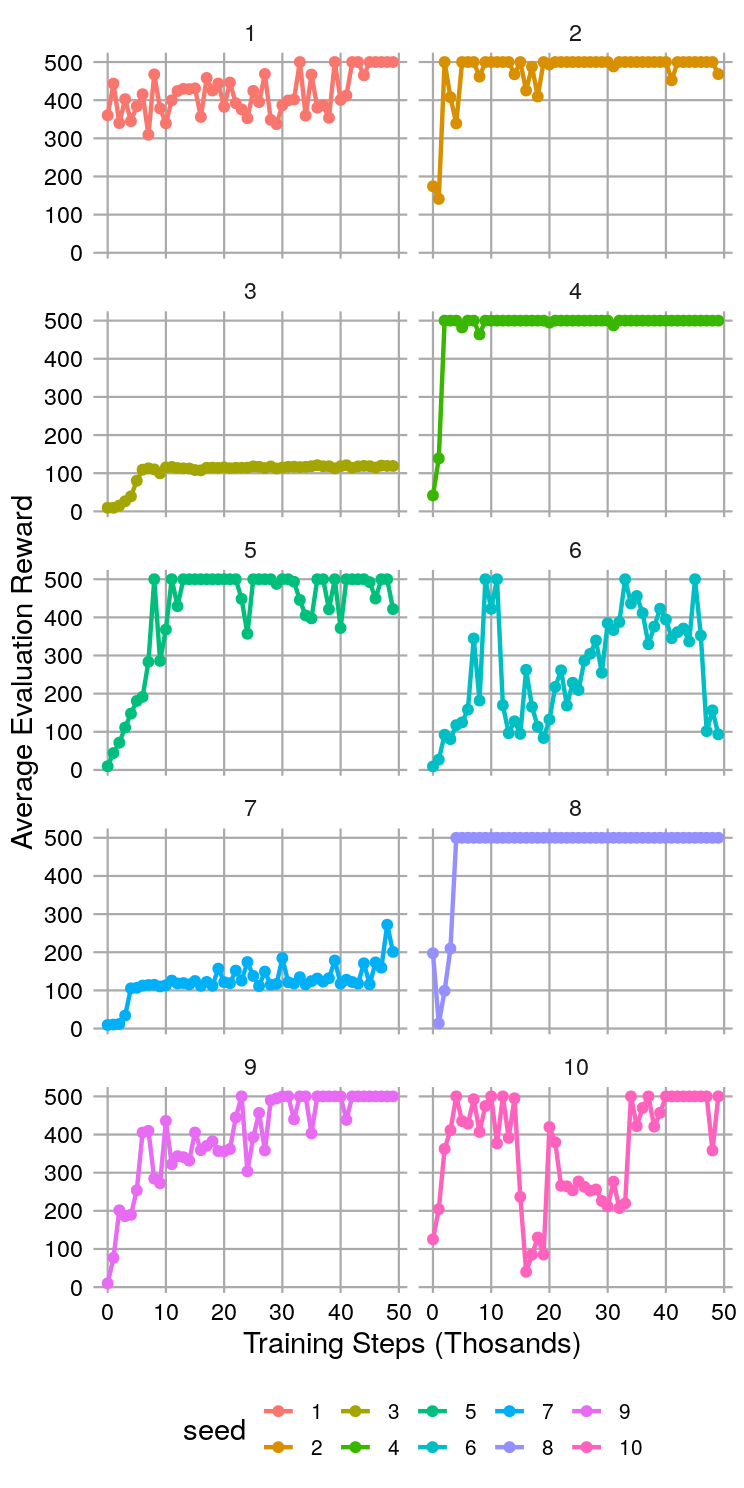
\includegraphics[scale=0.5]{PerDQNCartpole.png}
    }
    \subfloat[BNIG DQN]{
        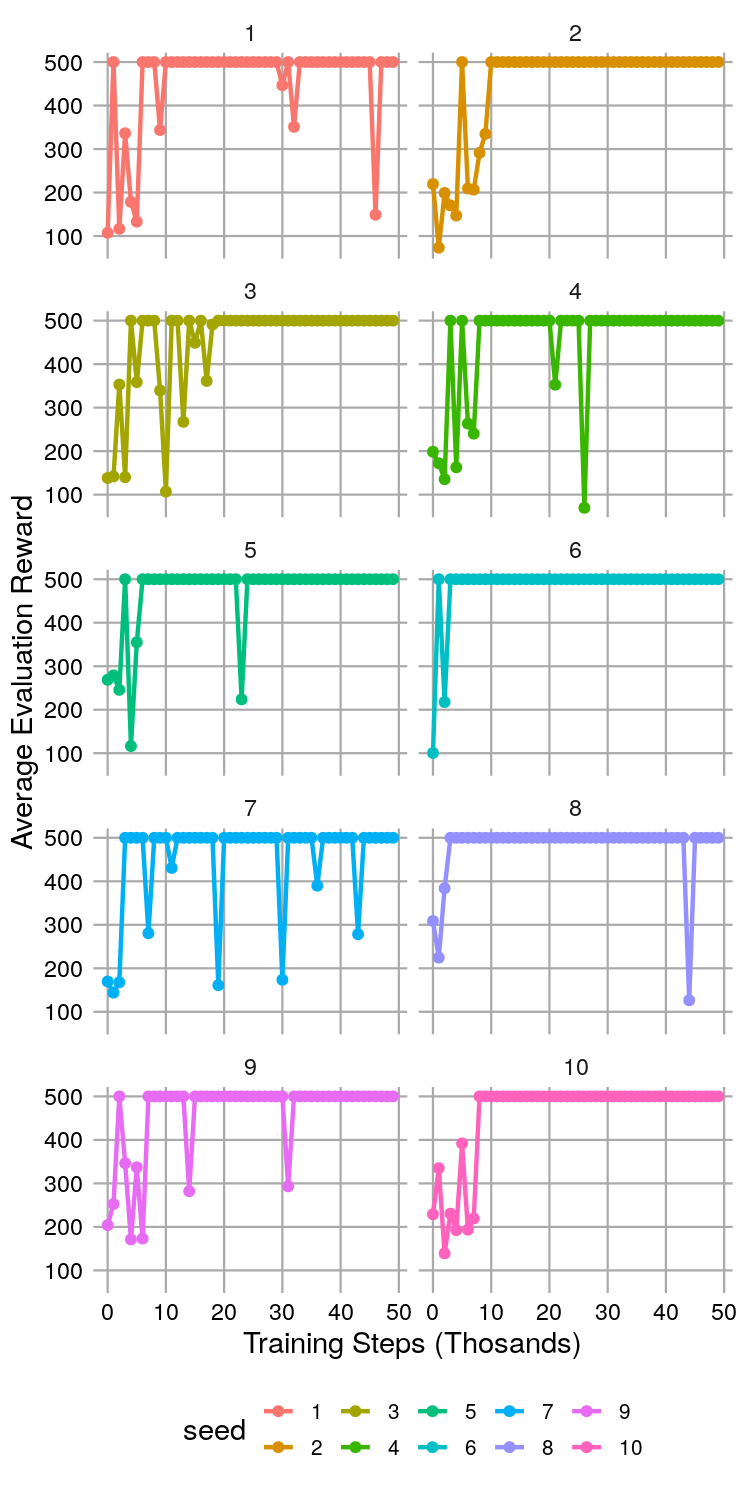
\includegraphics[scale=0.5]{PerBDQNCartpole.png}
    }
    \caption{\textbf{Per Seed DQN and BNIG DQN Performance on Cartpole}: Each color represents a new attempt. Note the unstable performance of DQN when it has found a good policy and that some attempts it never finds an optimal policy.}
    \label{fig:nn_per_cartpole}
\end{figure}

\subsection{Acrobot}

\begin{figure}[H]
    \centering
    \subfloat[DQN]{
        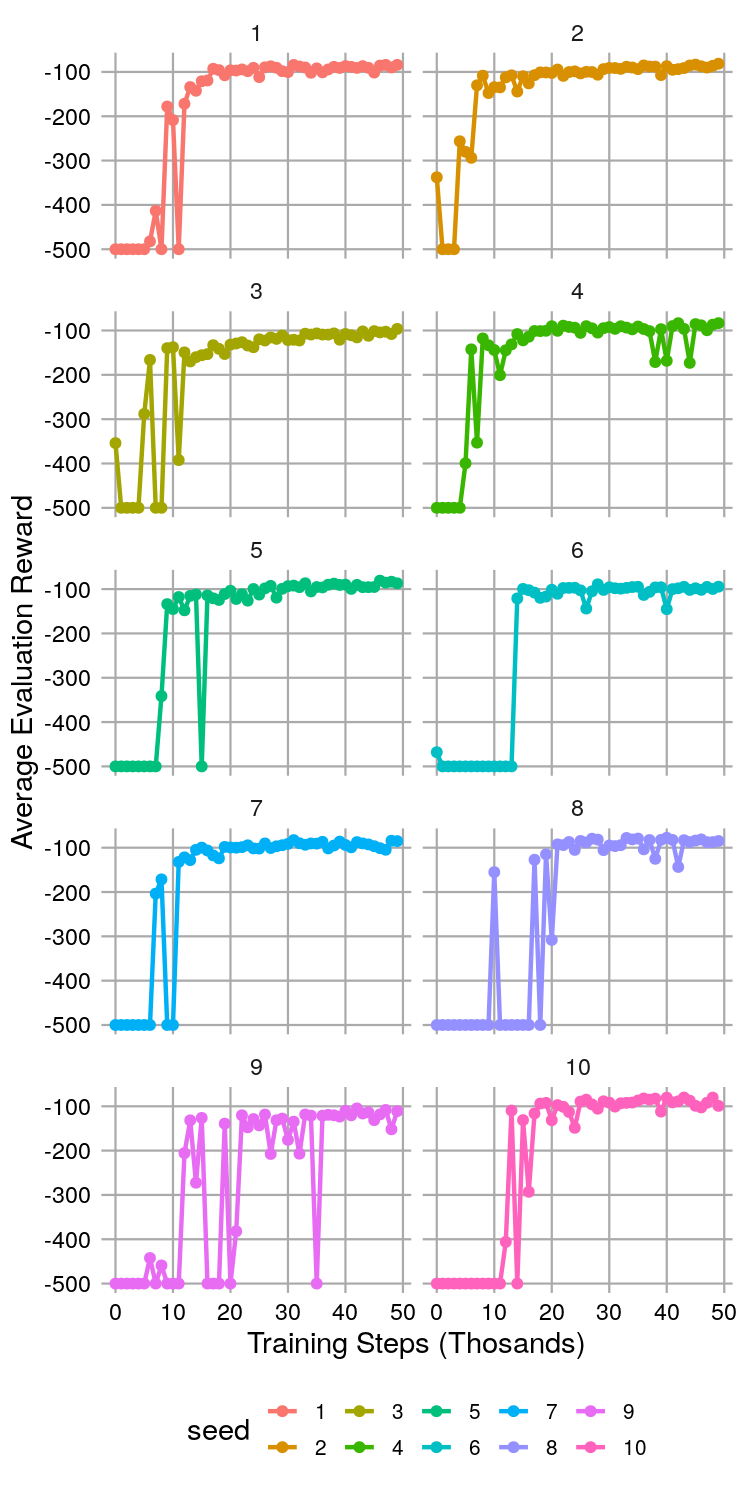
\includegraphics[scale=0.5]{PerDQNAcrobot.png}
    }
    \subfloat[BNIG DQN]{
        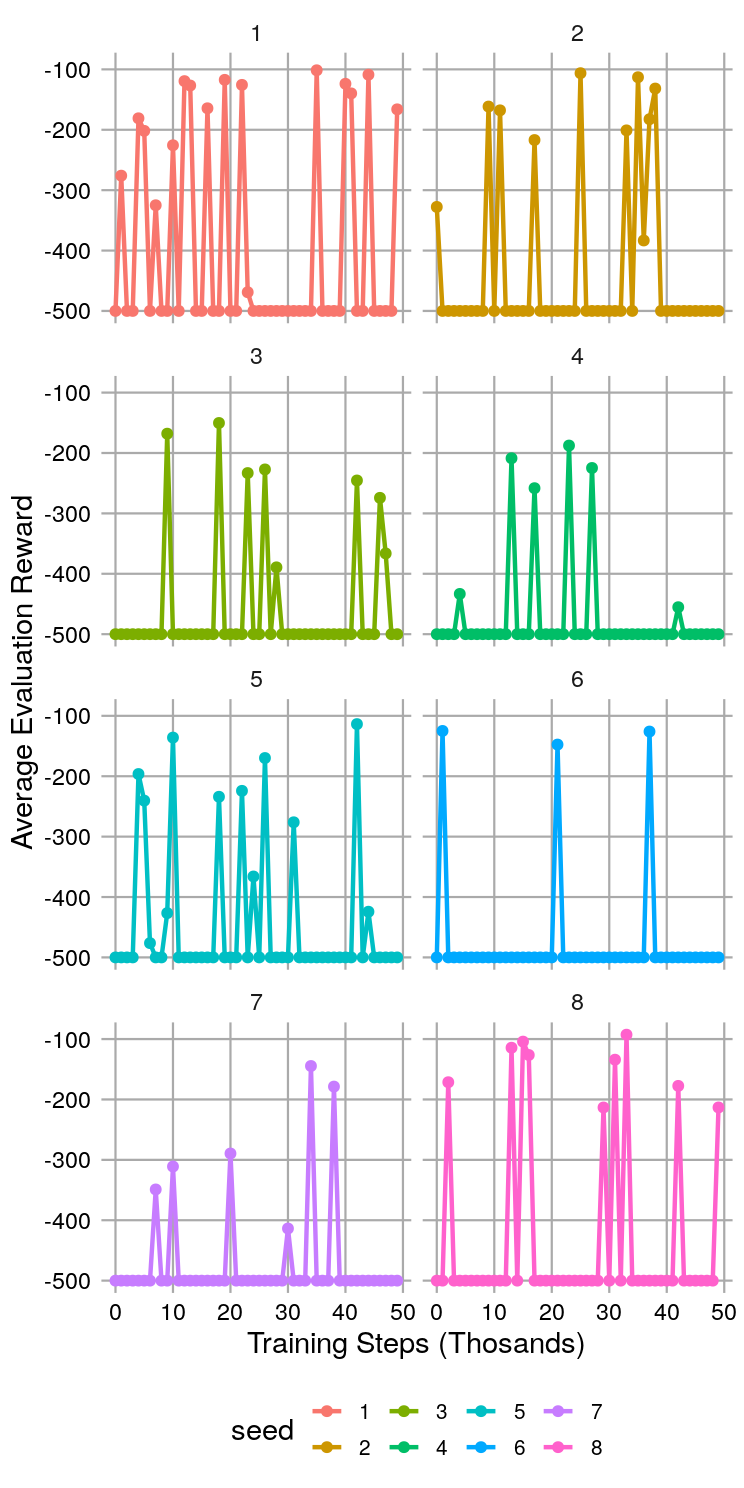
\includegraphics[scale=0.5]{PerBDQNAcrobot.png}
    }
    \caption{\textbf{Per Seed DQN and BNIG DQN Performance on Acrobot}: Each color represents a new attempt. The BNIG DQN occaisonaly finds a good policy, but is not able keep a stable policy.}
    \label{fig:nn_per_acrobot}
\end{figure}
